% LaTeX draft for SoftwareX submission (based on paper.md)
\documentclass[preprint,12pt]{elsarticle}
\usepackage{graphicx}
\usepackage{amsmath,amssymb}
\usepackage{hyperref}
\usepackage{booktabs}
\usepackage{longtable}

\begin{document}

\begin{frontmatter}
\title{PiXY: Pixel to stage-XY Coordinate Converter}

\author[inst1]{Yoshiaki KON}
\address[inst1]{Geological Survey of Japan (GSJ), National Institute of Advanced Industrial Science and Technology (AIST)}

\begin{abstract}
PiXY is open-source software that links target selection on microscopy images with physical positioning on an analytical instrument stage, reducing time in microanalysis workflows in geoscience and materials science. Conventionally, targets identified on microscope images must still be manually relocated on the analytical instrument, and this additional targeting step often becomes a major bottleneck.

PiXY addresses this bottleneck through two functions. First, it automatically extracts particle image coordinates $(u, v)$ by combining K-means color clustering with connected-component analysis. Second, it estimates an affine mapping from user-defined fiducial points using a least-squares method and converts the extracted image coordinates into physical stage coordinates $(X, Y, Z)$.
\end{abstract}

\begin{keyword}
particle detection 
\sep image segmentation 
\sep coordinate transformation 
\sep electron microscopy 
\sep open-source software
\end{keyword}

\end{frontmatter}

\section*{Summary}
\addcontentsline{toc}{section}{Summary}
% Summary kept as an unnumbered section (not part of main numbering)
PiXY is open-source software that links target selection on microscopy images with physical positioning on an analytical instrument stage, reducing time in microanalysis workflows in geoscience and materials science. (Summary text taken from the manuscript.)

\section{Introduction}
\subsection{Background}
Microanalysis instruments such as LA-ICP-MS, SEM-EDS, EPMA, and SIMS require reliable micrometer-scale targeting on solid sample surfaces. A common workflow is to image a sample in advance and then mount the same sample on an analytical instrument, where an operator adjusts an XYZ stage while viewing the instrument’s observation image.

\subsection{Problem statement and objectives}
Targeting on analytical instruments (Step 3 in common workflows) is often the bottleneck. PiXY aims to semi-automate the conversion from microscopy image coordinates to physical stage coordinates and provide instrument-ready outputs.

\subsection{Related work}
General-purpose image-analysis tools (e.g., ImageJ/FIJI, OpenCV) perform particle detection, while fiducial-based registration methods align images to stage coordinates. PiXY integrates these steps into a single GUI to streamline workflows.

\section{Software Description}
\subsection{Overview}
PiXY provides (1) automatic particle coordinate extraction and (2) affine mapping from image to stage coordinates, with interactive GUI controls and export options (CSV/clipboard).

\subsection{Key features and novelty}
\begin{itemize}
  \item K-means based clustering + connected-component centroid extraction for $(u,v)$ detection.
  \item Least-squares estimation of 2D→3D affine transformation from fiducial pairs.
  \item Interactive GUI (PySide6) for fiducial entry, residual inspection, and export.
  \item Distributed as Python source and a standalone Windows executable.
\end{itemize}

\subsection{Architecture and design}
Figure~\ref{fig:ui} shows the GUI. The code is modular: `Ui.py` (GUI), `CalcCentroid.py` (centroid extraction), `Util.py` (helpers and transformations), `rendering.py` (overlays), and `Main.py` (entry point).

\subsection{Dependencies and supported platforms}
PiXY is implemented in Python 3.8+ and depends on PySide6, OpenCV, NumPy; it is packaged as a Windows executable via PyInstaller. Source repository: \url{https://github.com/YoshiakiKON/PiXY}. Archive DOI: 10.5281/zenodo.18174474.

\begin{figure}
  \centering
  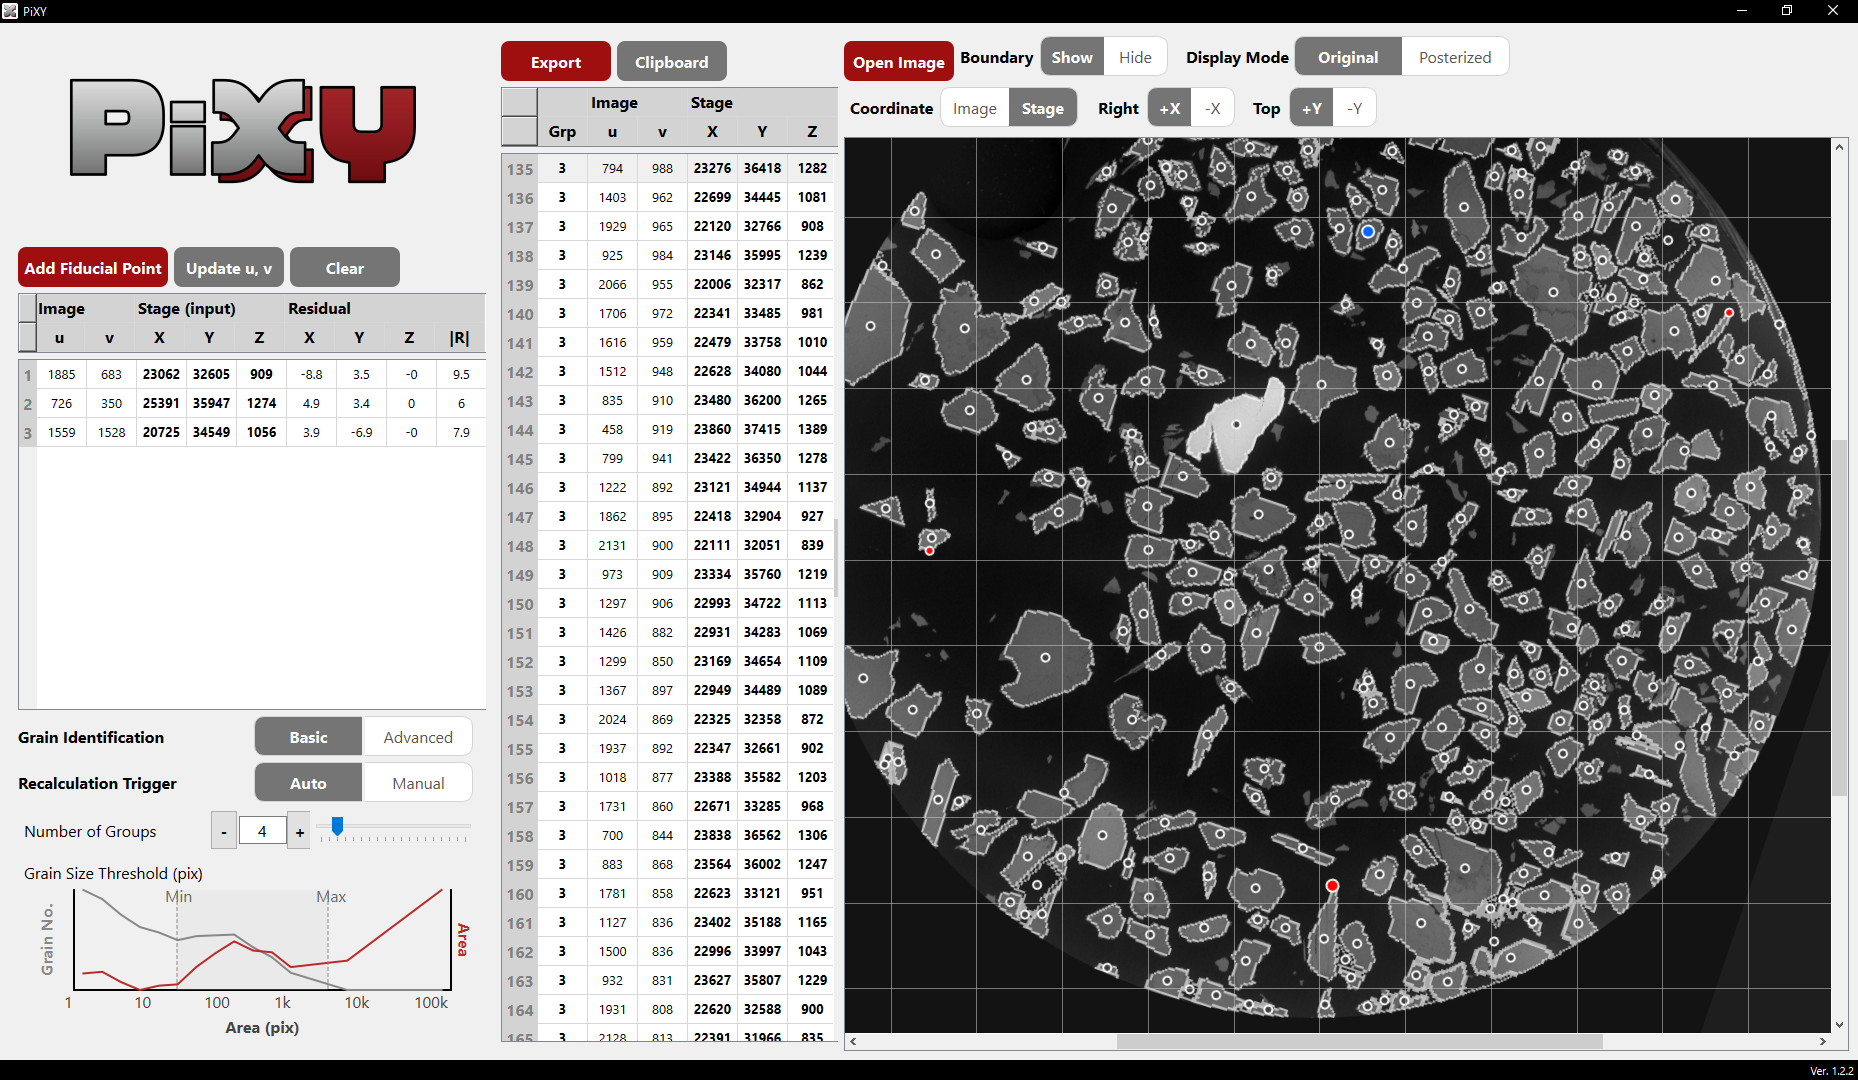
\includegraphics[width=0.8\textwidth]{documentation/images/fig_ui.png}
  \caption{PiXY GUI screenshot showing centroid overlays, fiducial points/residuals, and exportable coordinate tables.}
  \label{fig:ui}
\end{figure}

\section{Implementation}
\subsection{Algorithms and methods}
\subsubsection{Data structures}
Detections are represented as centroid coordinate lists; fiducial pairs are stored as paired image and stage coordinate tuples.

\subsubsection{Complexity / performance characteristics}
Centroid extraction is linear in the number of pixels for the clustering pass and connected-component labeling; preview operates on downscaled images for interactivity.

\subsection{Installation and usage}
Install requirements (example):
\begin{verbatim}
python -m pip install -r requirements.txt
python Main.py
\end{verbatim}
Windows users may run the provided executable.

\subsection{User interface and examples}
Users load an image, tune K (clusters) and area thresholds, click to add fiducials and enter measured stage coordinates, then export converted coordinates as CSV.

\section{Reproducibility and Testing}
\subsection{Validation experiments / benchmarks}
Validation used BSE images from JEOL JSM-6610LV and a laser‑ablation system (Raijin). Residual histograms for three- vs five-point fiducial configurations are shown in Figure~\ref{fig:residual}.

\begin{figure}
  \centering
  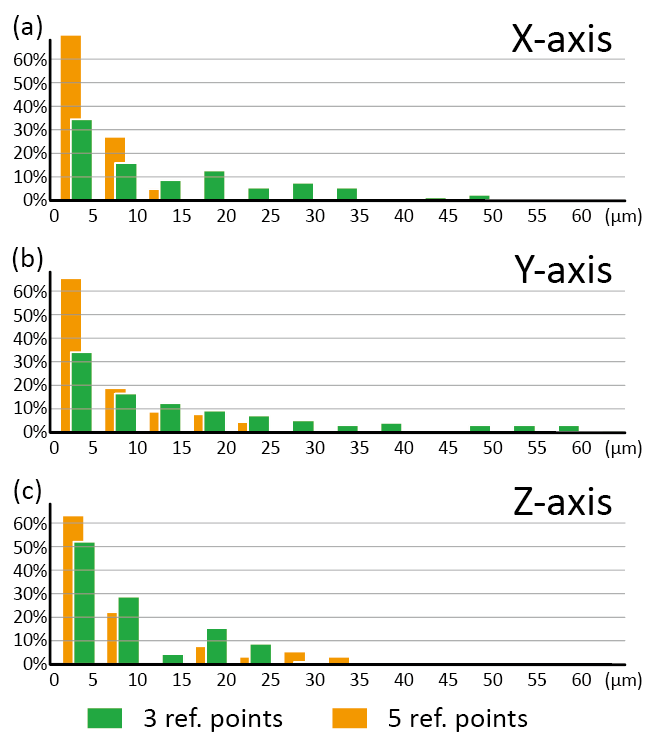
\includegraphics[width=0.8\textwidth]{documentation/images/fig_residual_hist.png}
  \caption{Residual histograms for each axis (X, Y, Z) comparing three vs. five fiducial points.}
  \label{fig:residual}
\end{figure}

\subsection{Test suite, CI, and expected outputs}
The repository includes unit tests for transformation routines and example images for manual verification. CI is recommended to run automated tests on core utilities.

\subsection{Availability of source code and archival DOI}
Repository: \url{https://github.com/YoshiakiKON/PiXY} (README.md, LICENSE.txt present). Archive DOI: 10.5281/zenodo.18174474.

\section{Impact, Limitations and Future Work}
\subsection{Intended users and applications}
Users of microanalysis instruments requiring micrometer targeting (geoscience, materials science laboratories).

\subsection{Known limitations}
Segmentation quality depends on image modality and specimen conditions; PiXY accepts pre-processed segmentation inputs when needed.

\subsection{Planned extensions}
Support for additional nonlinear registration models and tighter integration with instrument APIs may improve accuracy and automation.

\section{Metadata Table}
\begin{table}[ht]
\centering
\begin{tabular}{ll}
\toprule
Software title & PiXY: Pixel to stage-XY Coordinate Converter \\
Authors & Yoshiaki KON \\
Version & 1.2.3 \\
Repository URL & https://github.com/YoshiakiKON/PiXY \\
Archive DOI & 10.5281/zenodo.18174474 \\
License & MIT \\
Language & Python 3.8+ \\
Dependencies & PySide6, OpenCV, NumPy, PyInstaller \\
Release date & 29 January 2026 \\
\bottomrule
\end{tabular}
\caption{Required metadata for SoftwareX submission.}
\end{table}

\section{Glossary}
\begin{description}
  \item[Centroid:] Geometric center of a connected component region in a binarized/segmented image.
  \item[Fiducial point:] A distinctive feature on the specimen used to align image coordinates with stage coordinates.
  \item[Affine transformation:] A linear mapping that includes rotation, scaling, shear, and translation; used here to map $(x,y,1)$ to $(X,Y,Z)$.
  \item[K-means clustering:] Unsupervised clustering algorithm used to partition pixel values into K groups for segmentation.
\end{description}

\section{Acknowledgements}
This work was supported by JSPS KAKENHI (Grant Number: 25H00682). The authors also acknowledge the open-source scientific computing communities behind Python, OpenCV, NumPy, and PySide6.

\section{Author contributions: CRediT}
Conceptualization: Yoshiaki KON \\
Data curation: Yoshiaki KON \\
Formal analysis: Yoshiaki KON \\
Funding acquisition: Yoshiaki KON \\
Investigation: Yoshiaki KON \\
Methodology: Yoshiaki KON \\
Project administration: Yoshiaki KON \\
Resources: Yoshiaki KON \\
Software: Yoshiaki KON \\
Supervision: Yoshiaki KON \\
Validation: Yoshiaki KON \\
Visualization: Yoshiaki KON \\
Writing – original draft: Yoshiaki KON \\
Writing – review and editing: Yoshiaki KON

\section*{References}
\bibliographystyle{elsarticle-num}
\bibliography{paper}

\appendix
\section{Appendix A}
% If needed, add equations/tables referenced as Eq. (A.1), Table A.1, etc.

\end{document}
